\documentclass{beamer}

%Paquetes a usar
\usepackage{hyperref}
\usepackage{listings}
\usepackage{verbatim}
\usepackage{graphicx}
\usepackage[export]{adjustbox}
\usepackage{tikz}
\usetikzlibrary{positioning}

%Configuración del tema
\usetheme{Madrid}
\usecolortheme{whale}

%Estilo de código
\lstdefinestyle{micpp}{
	title=\lstname,
	language=C++,
	basicstyle=\tiny\ttfamily,
	breaklines=true, 
	keywordstyle=\color{blue},
	commentstyle=\color[rgb]{0,0.6,0},
  	identifierstyle=\color{orange},
 	stringstyle=\color{purple},
	tabsize=1,	
	escapechar=@,
}

\lstdefinestyle{miglsl}{
	title=\lstname,
	language=C++,
	basicstyle=\tiny\ttfamily,
	breaklines=true, 
	keywordstyle=\color{blue},
	commentstyle=\color[rgb]{0,0.6,0},
  	identifierstyle=\color{orange},
 	stringstyle=\color{purple},
	tabsize=1,	
	escapechar=@,
	morekeywords={
		vec2, vec3, vec4,
		mat2, mat3, mat4,
		uniform, sampler2d, sampler2D
	}
}

%Estilo Tikz
\tikzstyle{ZuazoBase}=[rectangle, draw=blue!60, fill=blue!5, very thick, minimum width=18mm, minimum height=18mm, font=\large]
\tikzstyle{SourceBase}=[rectangle, draw=red!60, fill=red!5, very thick, minimum width=18mm, minimum height=18mm, font=\large]
\tikzstyle{ConsumerBase}=[rectangle, draw=green!60, fill=green!5, very thick, minimum width=18mm, minimum height=18mm, font=\large]
\tikzstyle{SourcePad}=[rectangle, draw=red!60, fill=red!5, thick, minimum height=3mm, font=\tiny]
\tikzstyle{ConsumerPad}=[rectangle, draw=green!60, fill=green!5, thick, minimum height=3mm, font=\tiny]
\tikzstyle{Flecha}=[->, line width=1.5]

%Directorio de gráficos
\graphicspath{ {../images/} }

%Metadata
\title{Zuazo}
\subtitle{Librería para manipular video en tiempo real}
\author{Oier Lauzirika Zarrabeitia}
\institute[]{Estudiante de Ingeniería de Sonido e Imagen en ETSIST-UPM}
\date[FF del CUSL 13]{Fase final del CUSL 13, 10/05/2019} 

%Al cominezo de cada sección
\AtBeginSection[]
{
	\begin{frame}
		\frametitle{Contenidos}
  		\tableofcontents[currentsection]
	\end{frame}
}

\beamertemplatenavigationsymbolsempty

%Comenzamos con la presentación
\begin{document}

%
%Página del título
%

\begin{frame}
	\maketitle
	\begin{columns}
		\column{0.5\textwidth} 
\includegraphics[width=\textwidth]{zuazo_logo}
		\column{0.5\textwidth} 
\includegraphics[width=\textwidth]{cusl13_logo}
	\end{columns}
\end{frame}

%
% Sección de Introducción
%
\section{Introducción}

%¿Qué es Zuazo?
\begin{frame} \frametitle{¿Qué es Zuazo?}
	\begin{itemize}
		\item{Una librería para manipular video en tiempo real}
		\item{Escrita en C++17, incluyendo la API}
		\item{Soporta distribuciones GNU/Linux basadas en Debian} 
		\item{Emplea aceleración por GPU en la medida de lo posible}
		\item{Es seguro en hilos (thread safe)}
		\item{Relativamente fácil de usar}
	\end{itemize}
\end{frame}

%¿Por que decidí empezar Zuazo?
\begin{frame} \frametitle{¿Por que decidí empezar Zuazo?}
	\begin{block}{Ya existían alternativas}
		\begin{itemize}
			\item{MLT (Media Lovin' Toolkit)}
			\item{GStreamer}
			\item{\ldots}
		\end{itemize}
	\end{block}
	\textbf{Entonces, ¿Por qué?}
	\begin{itemize}
		\item{Falta de documentación (MLT)}
		\item{Diseñada para C, API compleja (GStreamer)}
		\item{Sin énfasis en manipular video por hardware (Ambas)} 
		\item{Sin énfasis en tiempo real (MLT)} 
		\item{Ganas de hacer un proyecto relacionado con manipulación de video}
	\end{itemize}
\end{frame}

%Librerias de terceros
\begin{frame} \frametitle{Librerías de terceros}
	\begin{itemize}
		\item{Librería estándar de C++}
		\item{OpenGL ES 3.0}
		\item{GLFW3 (a reemplazar por SDL2)}
		\item{FFmpeg}
		\item{Magick++}
		\item{V4L2}
	\end{itemize}
\end{frame}


%
% Dinámica de Zuazo
%
\section{Dinámica de Zuazo}

\begin{frame}[allowframebreaks, fragile] \frametitle{Dináminca general}
	\begin{figure}
		 \begin{itemize}
			\item{Todo se encuentra en el espacio de nombres (o en un subespacio de nombres de)  \texttt{Zuazo}, o abreviado \texttt{zz}}	
			\item{Para poder empezar a usar Zuazo, hay que inicializarlo con \texttt{Zuazo::init()}} 
			\item{Al terminar, conviene liberar todo con \texttt{Zuazo::terminate()} (No hacerlo es de malas personas)} 
			\item{Antes de llamar a \texttt{Zuazo::terminate()} \textbf{TODOS} los objetos de Zuazo deben haberse destruido o cerrado} 
			\item{\textbf{TODOS} los comandos (excepto  \texttt{init()} y  \texttt{terminate()}) se deben de ordenar entre un  \texttt{begin()} y un  \texttt{end()} o equivalente, que llamaremos "contexto"}
			\item{Declarar un objeto de la clase \texttt{zz::Context}, es equivalente a hacer \texttt{begin()} y \texttt{end()} (Cuando  \texttt{zz::Context} se construye se ejecuta  \texttt{begin()} y cuando se destruye se ejecuta  \texttt{end()})}
			\item{Sólo puede haber un contexto activo en todo momento (está protegido con un mutex)} 
			\item{Mientras que haya un contexto activo, el renderizado de Zuazo estará pausado (minimizar tiempo con contexto activo)} 	
			\item{Todos los cambios realizados en un mismo contexto ocurrirán en un mismo fotograma} 
		\end{itemize}
		\begin{lstlisting}[style=micpp, frame=single]
			zz::init(); //Inicializa Zuazo

			zz::begin(); //Comenzamos a ordernar cosas a Zuazo
			//[...]
			zz::end(); //Hemos terminado de momento

			if(){
				zz::Context ctx; //La vida de este objeto representa un begin() y end()
				//[...]
			}

			zz:terminate();//Libera todos los recursos adquiridos por Zuazo
		\end{lstlisting}
	\end{figure}
\end{frame}

\begin{frame}[fragile] \frametitle{Source / Consumer / Processor}
	\begin{columns}
		\begin{column}{0.48\textwidth}
			\begin{block}{Source}
				\center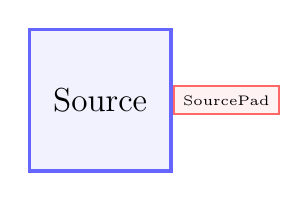
\begin{tikzpicture}
					\node[ZuazoBase]	(source)							{Source};
					\node[SourcePad]	(source_pad)	[right=0cm of source]	{SourcePad};
				\end{tikzpicture}
				\begin{itemize}
					\item{Al menos un SourcePad}
					\item{Ningún ConsumerPad}
				\end{itemize}
			\end{block}
		\end{column}
		\begin{column}{0.48\textwidth}
			\begin{block}{Consumer}
				\center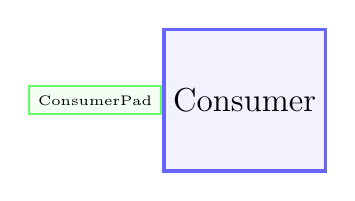
\begin{tikzpicture}
					\node[ZuazoBase]		(consumer)							{Consumer};
					\node[ConsumerPad]	(consumer_pad)	[left=0cm of consumer]	{ConsumerPad};
				\end{tikzpicture}
				\begin{itemize}
					\item{Al menos un ConsumerPad}
					\item{Ningún SourcePad}
				\end{itemize}
			\end{block}
		\end{column}
	\end{columns}
	\begin{block}{Processor} 
		\center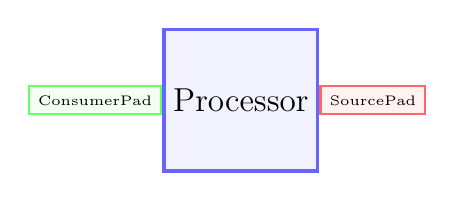
\begin{tikzpicture}
			\node[ZuazoBase]		(processor)							{Processor};
			\node[ConsumerPad]	(consumer_pad)	[left=0cm of processor]	{ConsumerPad};
			\node[SourcePad]		(source_pad)		[right=0cm of processor]	{SourcePad};
		\end{tikzpicture}
		\begin{itemize}
			\item{El resto}
		\end{itemize}
	\end{block}
\end{frame}

\begin{frame}[allowframebreaks, fragile] \frametitle{Dináminca de flujo}
	\begin{figure} {Un "Consumer" puede ser alimentado de un "Source"}
		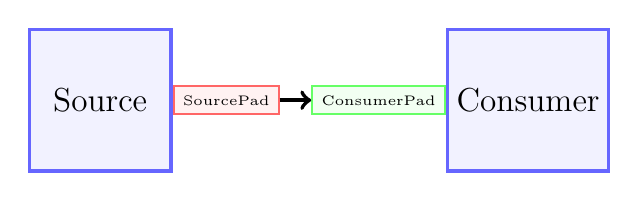
\begin{tikzpicture}
			%Nodos
			\node[ZuazoBase]		(source)									{Source};
			\node[SourcePad]		(source_src)		[right = 0cm of source]		{SourcePad};

			\node[ConsumerPad]	(consumer_cons)	[right=4mm of source_src]	{ConsumerPad};
			\node[ZuazoBase]		(consumer)		[right=0cm of consumer_cons]	{Consumer};

			%Lineas
			\draw[Flecha] (source_src.east) -- (consumer_cons.west);

		\end{tikzpicture}
		\begin{lstlisting}[style=micpp, frame=single]
			FooSource source;
			FooConsumer consumer;
		
			//Los 3 son equivalentes
			consumer.consumerPad << source.sourcePad;
			source.sourcePad >> consumer.consumerPad;
			consumer.setSource(&source.sourcePad);
		\end{lstlisting}
	\end{figure}
	
	\begin{figure} {Los elementos pueden estar sin "conectarse"}
		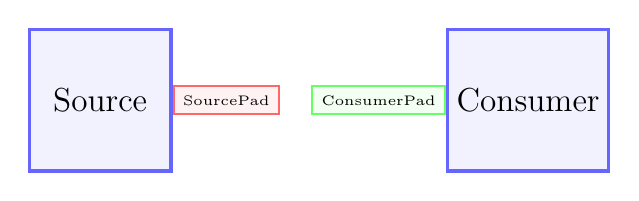
\begin{tikzpicture}
			%Nodos
			\node[ZuazoBase]		(source)									{Source};
			\node[SourcePad]		(source_src)		[right = 0cm of source]		{SourcePad};

			\node[ConsumerPad]	(consumer_cons)	[right=4mm of source_src]	{ConsumerPad};
			\node[ZuazoBase]		(consumer)		[right=0cm of consumer_cons]	{Consumer};

		\end{tikzpicture}
		\begin{lstlisting}[style=micpp, frame=single]
			consumer.consumerPad << nullptr; //Para dejar de alimentar un Consumer
		\end{lstlisting}
	\end{figure}

	\begin{figure}  {Un "Source" puede alimentar varios "Consumer"}
		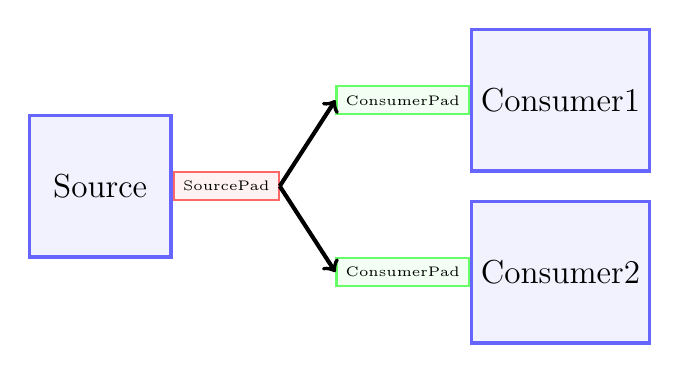
\begin{tikzpicture}
			%Nodos
			\node[ZuazoBase]		(source)										{Source};
			\node[SourcePad]		(source_src)		[right = 0cm of source]			{SourcePad};

			\node[ConsumerPad]	(consumer1_cons)	[above right=10mm of source_src] 	{ConsumerPad};
			\node[ZuazoBase]		(consumer1)		[right=0cm of consumer1_cons]	{Consumer1};

			\node[ConsumerPad]	(consumer2_cons)	[below right=10mm of source_src]	{ConsumerPad};
			\node[ZuazoBase]		(consumer2)		[right=0cm of consumer2_cons]	{Consumer2};

			%Lineas
			\draw[Flecha] (source_src.east) -- (consumer1_cons.west);
			\draw[Flecha] (source_src.east) -- (consumer2_cons.west);

		\end{tikzpicture}
		\begin{lstlisting}[style=micpp, frame=single]
			consumer1.consumerPad << source.sourcePad;
			consumer2.consumerPad << source.sourcePad;
		\end{lstlisting}
	\end{figure}

	\begin{figure} {Puede haber varios "pipelines" independientes}
		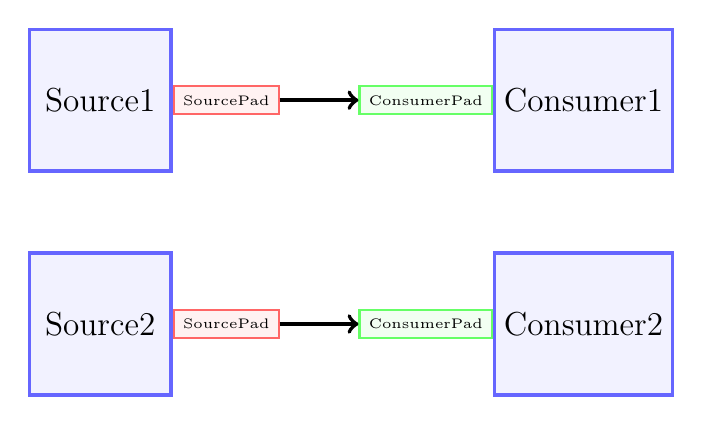
\begin{tikzpicture}
			%Nodos
			\node[ZuazoBase]		(source1)									{Source1};
			\node[SourcePad]		(source1_src)		[right = 0cm of source1]		{SourcePad};

			\node[ZuazoBase]		(source2)			[below =1cm of source1]		{Source2};
			\node[SourcePad]		(source2_src)		[right = 0cm of source2]		{SourcePad};

			\node[ConsumerPad]	(consumer1_cons)	[right=10mm of source1_src] 	{ConsumerPad};
			\node[ZuazoBase]		(consumer1)		[right=0cm of consumer1_cons]{Consumer1};

			\node[ConsumerPad]	(consumer2_cons)	[right=10mm of source2_src] 	{ConsumerPad};
			\node[ZuazoBase]		(consumer2)		[right=0cm of consumer2_cons]{Consumer2};

			%Lineas
			\draw[Flecha] (source1_src.east) -- (consumer1_cons.west);
			\draw[Flecha] (source2_src.east) -- (consumer2_cons.west);

		\end{tikzpicture}

		\begin{lstlisting}[style=micpp, frame=single]
			consumer1.consumerPad << source1.sourcePad;
			consumer2.consumerPad << source2.sourcePad;
		\end{lstlisting}
	\end{figure}

	\begin{figure}  {Los "pipelines" pueden tener cualquier longitud}
		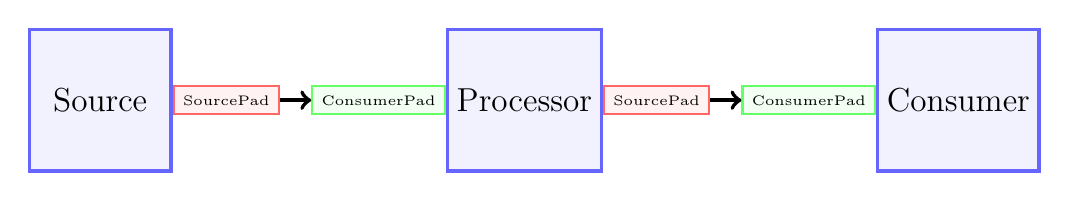
\begin{tikzpicture}
			%Nodos
			\node[ZuazoBase]		(source)									{Source};
			\node[SourcePad]		(source_src)		[right = 0cm of source]		{SourcePad};

			\node[ConsumerPad]	(processor_cons) 	[right = 4mm of source_src]	{ConsumerPad};
			\node[ZuazoBase]		(processor)		[right = 0cm of processor_cons]	{Processor};
			\node[SourcePad]		(processor_src)		[right = 0cm of processor)]	{SourcePad};	

			\node[ConsumerPad]	(consumer_cons)	[right=4mm of processor_src]	{ConsumerPad};
			\node[ZuazoBase]		(consumer)		[right=0cm of consumer_cons]	{Consumer};

			%Lineas
			\draw[Flecha] (source_src.east) -- (processor_cons.west);
			\draw[Flecha] (processor_src.east) -- (consumer_cons.west);

		\end{tikzpicture}
		\begin{lstlisting}[style=micpp, frame=single]
			consumer.consumerPad << processor.sourcePad;
			processor.consumerPad << source.sourcePad;
		\end{lstlisting}
	\end{figure}

	\begin{figure}  {Los "pipelines" pueden tener recursividad (hasta un nivel finito)}
		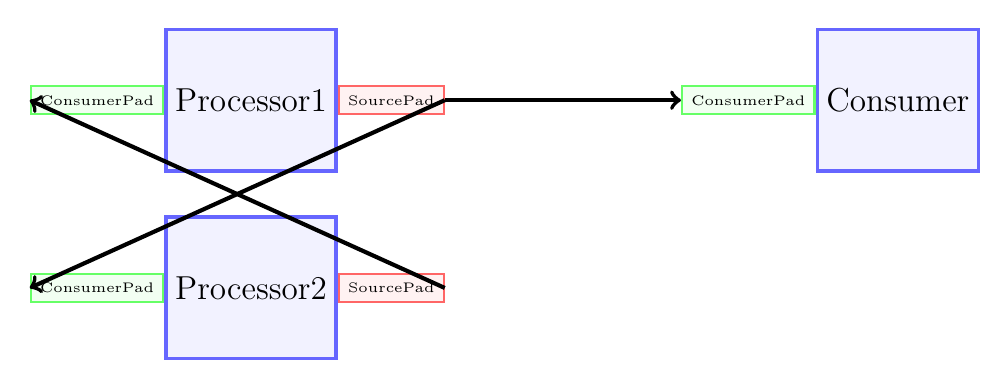
\begin{tikzpicture}
			%Nodos
			\node[ConsumerPad]	(processor1_cons) 								{ConsumerPad};
			\node[ZuazoBase]		(processor1)		[right = 0cm of processor1_cons]	{Processor1};
			\node[SourcePad]		(processor1_src)	[right = 0cm of processor1)]		{SourcePad};	

			\node[ConsumerPad]	(processor2_cons) 	[below = 2cm of processor1_cons]	{ConsumerPad};
			\node[ZuazoBase]		(processor2)		[right = 0cm of processor2_cons]	{Processor2};
			\node[SourcePad]		(processor2_src)	[right = 0cm of processor2)]		{SourcePad};	

			\node[ConsumerPad]	(consumer_cons)	[right=3cm of processor1_src]		{ConsumerPad};
			\node[ZuazoBase]		(consumer)		[right=0cm of consumer_cons]		{Consumer};

			%Lineas
			\draw[Flecha] (processor2_src.east) -- (processor1_cons.west);
			\draw[Flecha] (processor1_src.east) -- (processor2_cons.west);
			\draw[Flecha] (processor1_src.east) -- (consumer_cons.west);

		\end{tikzpicture}
		\begin{lstlisting}[style=micpp, frame=single]
			consumer.consumerPad << processor1.sourcePad;
			processor1.consumerPad << processor2.sourcePad;
			processor2.consumerPad << processor1.sourcePad;
			processor1.setMaxRecursion(10);
			processor2.setMaxRecursion(10); //En caso de ser distinto, se escojera el minimo
		\end{lstlisting}
	\end{figure}

	\begin{figure}  {Un "Consumer" \textbf{NO} puede tener varios "Source"} 
		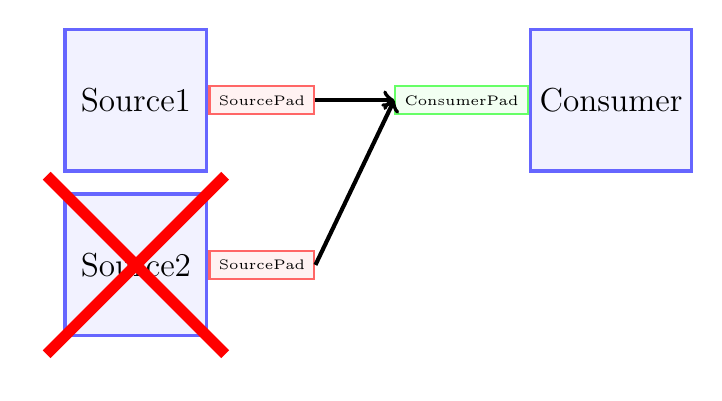
\begin{tikzpicture}
			%Nodos
			\node[ZuazoBase]		(source1)									{Source1};
			\node[SourcePad]		(source1_src)		[right = 0cm of source1]		{SourcePad};

			\node[ZuazoBase]		(source2)			[below =0.25cm of source1]		{Source2};
			\node[SourcePad]		(source2_src)		[right = 0cm of source2]		{SourcePad};

			\node[ConsumerPad]	(consumer_cons)	[right=10mm of source1_src] 	{ConsumerPad};
			\node[ZuazoBase]		(consumer)		[right=0cm of consumer_cons]	{Consumer};

			%Lineas
			\draw[Flecha] (source1_src.east) -- (consumer_cons.west);
			\draw[Flecha] (source2_src.east) -- (consumer_cons.west);
			
			%X
			\node[above right = 3mm of source2] (a) {};
			\node[below left = 3mm of source2] (b) {};
			\node[above left = 3mm of source2] (c) {};
			\node[below right = 3mm of source2] (d) {};
			\draw[-, color=red, line width=4] (a) -- (b);
			\draw[-, color=red, line width=4] (c) -- (d);

		\end{tikzpicture}
		\begin{lstlisting}[style=micpp, frame=single]
			consumer.consumerPad << source1.sourcePad; //No sirve para nada, ya que acto seguido se "machacara"
			consumer.consumerPad << source2.sourcePad; //Aqui se "machaca" la fuente anterior
		\end{lstlisting}
	\end{figure}
\end{frame}

\begin{frame}[fragile] \frametitle{Clases base de Zuazo}
	\begin{figure} 
		
\begin{tikzpicture}
			\node[ZuazoBase]		(zuazo_base)											{ZuazoBase};
		\end{tikzpicture}
		
\begin{tikzpicture}
			\node[ZuazoBase]		(video_base)											{VideoBase};
		\end{tikzpicture}
	\end{figure}
	\begin{figure} 
		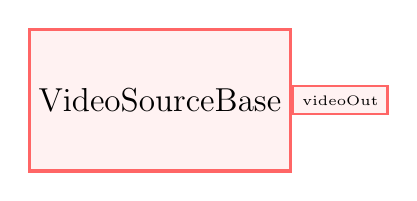
\begin{tikzpicture}
			\node[SourceBase]		(video_source_base)										{VideoSourceBase};
			\node[SourcePad]		(video_source_pad)		[right=0cm of video_source_base]		{videoOut};
		\end{tikzpicture}
	\end{figure}
	\begin{figure} 
		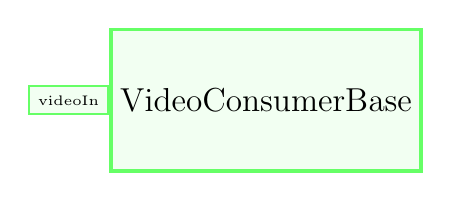
\begin{tikzpicture}
			\node[ConsumerBase]	(video_consumer_base)									{VideoConsumerBase};
			\node[ConsumerPad]	(video_consumer_pad)	[left=0cm of video_consumer_base]		{videoIn};
		\end{tikzpicture}
	\end{figure}
\end{frame}

%
% Documentación
%
\section{Documentación}

%Documentación
\begin{frame} \frametitle{Documentación}
	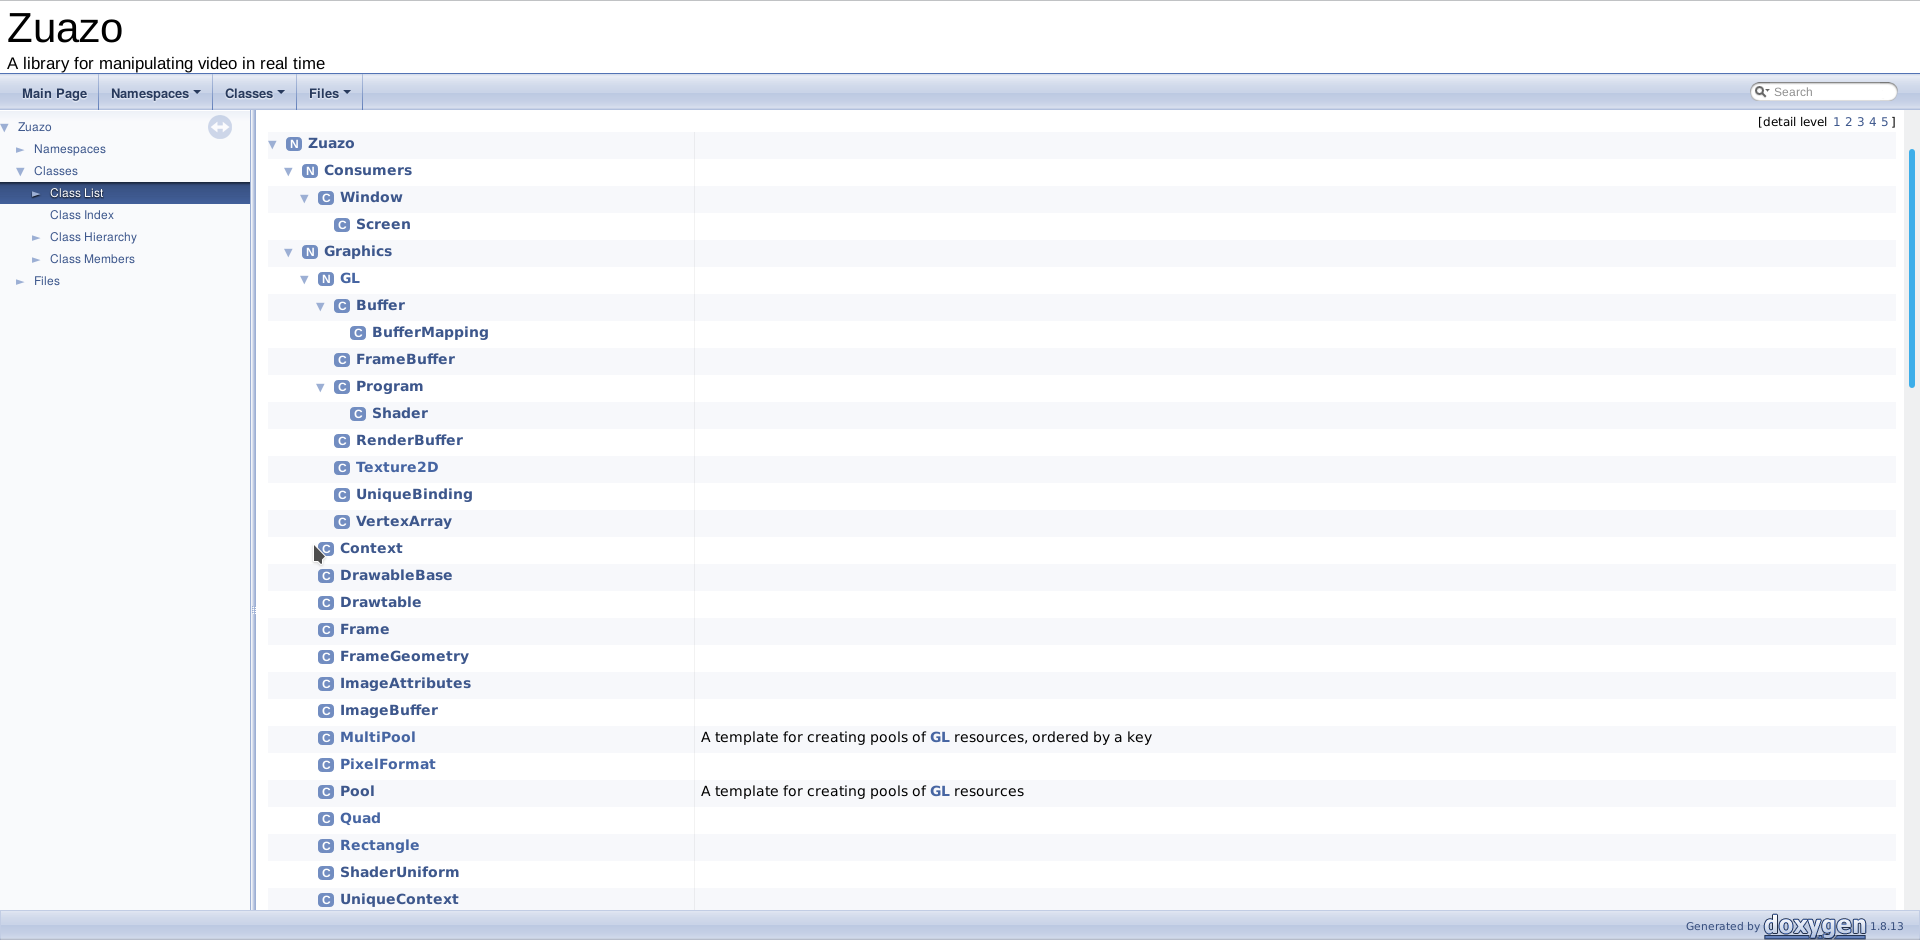
\includegraphics[width=\textwidth]{doxy1} 
\end{frame}

\begin{frame}[allowframebreaks] \frametitle{ZuazoBase}
	\center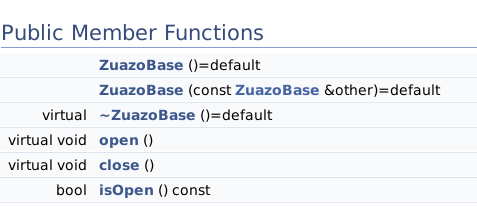
\includegraphics[width=\textwidth]{zuazo_base} 
\end{frame}

\begin{frame}[allowframebreaks] \frametitle{API general del video}
\begin{center}
	\center\large\bf VideoBase\\
	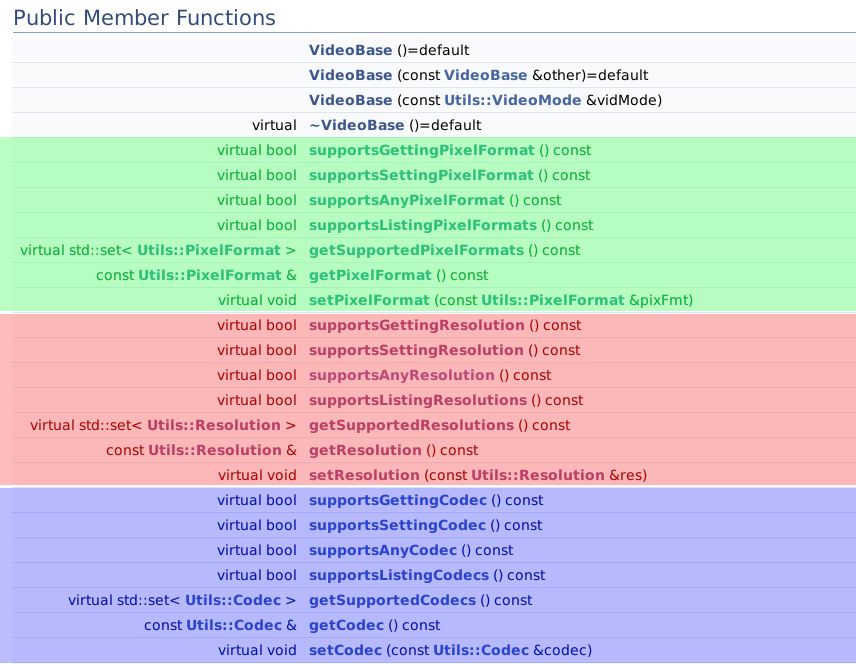
\includegraphics[height=0.75\textheight]{video_base1} 
	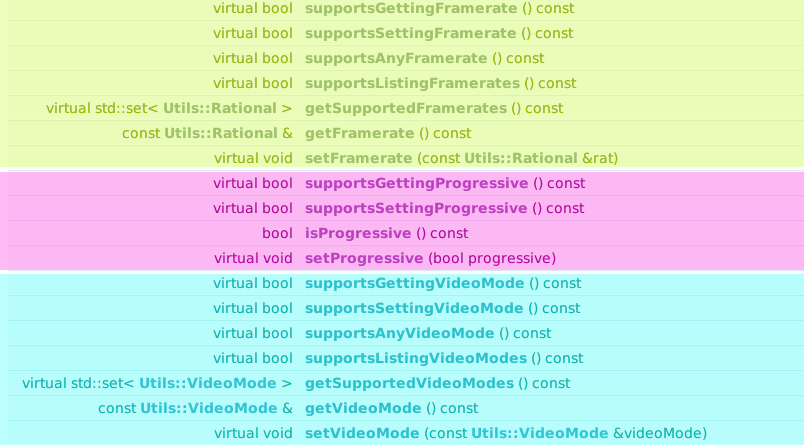
\includegraphics[width=\textwidth]{video_base2} 
	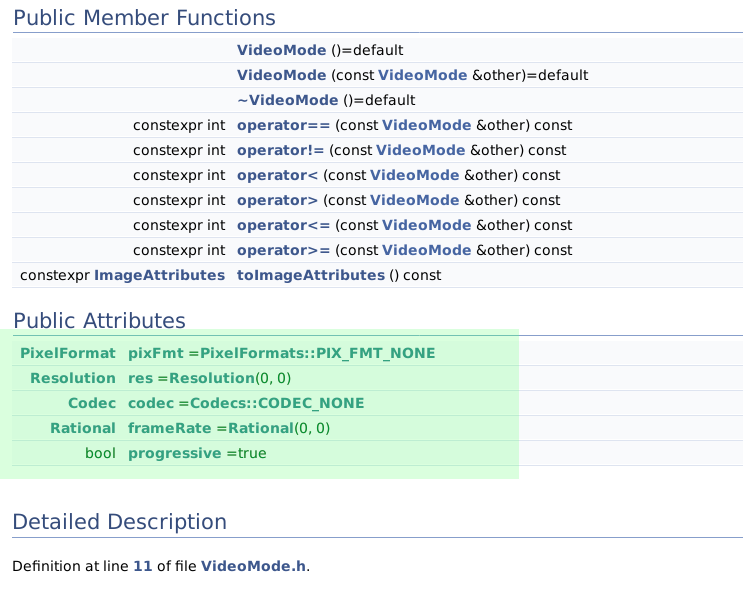
\includegraphics[height=0.8\textheight]{video_mode_struct} 
	\center\large\bf VideoConsumer\\
	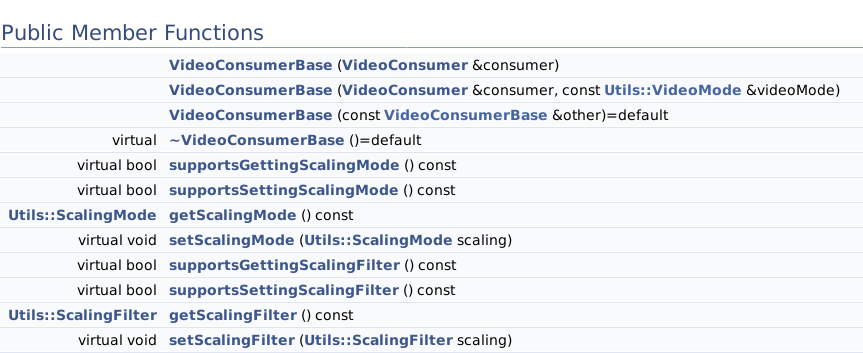
\includegraphics[width=\textwidth]{video_consumer} 
	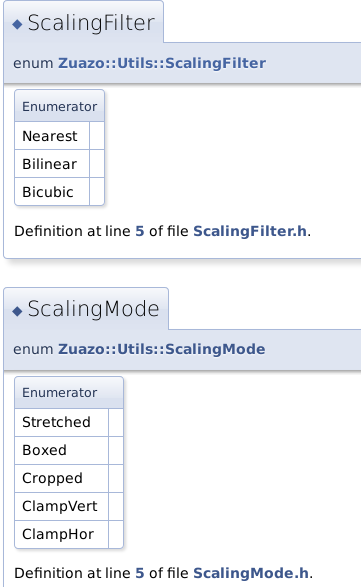
\includegraphics[height=0.8\textheight]{scaling} 
\end{center}
\end{frame}

%
% E/S disponible y "procesadores"
%
\section{E/S disponible y "procesadores"}

%Entradas de video disponibles
\begin{frame}[t] \frametitle{Entradas de video disponibles}
	\begin{itemize}
		\item{Archivos de video} \pause
		\item{Archivos de imágenes} \pause
		\item{Dispositivos compatible con V4L2}
	\end{itemize}
\end{frame}

%Salidas de video disponibles
\begin{frame}[t] \frametitle{Salidas de video disponibles}
	\begin{itemize}
		\item{Ventana}
		\item{Monitor}
	\end{itemize}
\end{frame}

%Efectos basados en shaders de fragmento
\begin{frame}[t] \frametitle{Efectos basados en shaders de fragmento}
	\begin{itemize}
		\item{Corrección de tono, saturación y luminosidad (HSL)} \pause
		\item{Corrección de brillo y contraste} \pause
		\item{Color a escala de grises} \pause
		\item{Chroma key}  \pause
		\item{Representación en luminancia del canal alpha}  \pause
		\item{Invertir color} \pause
		\item{A definir por el usuario}
	\end{itemize}
\end{frame}

%Compositor
\begin{frame}[t] \frametitle{Compositor}
	\begin{itemize}
		\item{Combina varias fuentes en una sola salida} \pause
		\item{Se organiza en capas}  \pause
		\item{Entorno 3D: Cámara y capas transformables en el espacio}
	\end{itemize}
\end{frame}

%
% Ejemplos
%
\section{Ejemplos}

%¡Hola  Mundo!
\begin{frame}[t, allowframebreaks] \frametitle{Programa "¡Hola Mundo!"}
	\lstinputlisting[style=micpp]{../code/HolaMundo.cpp}
\end{frame}

%Creación de shaders de fragmento
\begin{frame}[t, allowframebreaks] \frametitle{Creación de shaders de fragmento}
	\lstinputlisting[style=miglsl]{../code/quantize.glsl}
	\lstinputlisting[style=micpp]{../code/Cuantizar.h}
	\lstinputlisting[style=micpp]{../code/Cuantizar.cpp}
	\lstinputlisting[style=micpp]{../code/CuantizarApp.cpp}	
\end{frame}

%
% Conclusiones
%
\section{Futuro}

%Bugs
\begin{frame} \frametitle{Bugs}
	\begin{itemize}
		\item{Transparencia independiente del orden (OIT) en el compositor}
		\item{La entrada de V4L2 funciona mal a resoluciones bajas (Posible bug de FFmpeg)}
	\end{itemize}
\end{frame}

%Cosas por hacer a corto plazo
\begin{frame}[t] \frametitle{Cosas por hacer a corto plazo}
	\begin{itemize}
		\begin{item}
			Cambiar librería de ventanas (GLFW3 por SDL2)
			\begin{itemize}
				\item{Permite integración con QT}
				\item{Reescribir la clase "Window", con el debido soporte de pantalla completa y gestión de eventos}
			\end{itemize}
		\end{item}
		\begin{item}
			Completar efectos ya existentes
			\begin{itemize}
				\item{Mejor gestión de parámetros}
				\item{Mayor número de parámetros}
			\end{itemize}
		\end{item}
		\begin{item}
			Más tipos de capas en el compositor
			\begin{itemize}
				\item{Capa de video deformable}
				\item{Formas geométricas}
			\end{itemize}
		\end{item}
		\begin{item}
			Terminar de codificar los métodos \texttt{init()} y \texttt{terminate()}
		\end{item}
		\begin{item}
			Añadir las extensiones que faltan a \texttt{videoSourceFromFile([...])}
		\end{item}
		\begin{item}
			Añadir los comentarios de Doxygen
		\end{item}
		\begin{item}
			Unificar los formatos de pixeles y demás
		\end{item}
	\end{itemize}
\end{frame}

%Cosas por hacer a largo plazo
\begin{frame}[t] \frametitle{Cosas por hacer a largo plazo}
	\begin{itemize}
		\begin{item}
			Añadir más entradas y salidas
			\begin{itemize}
				\item{Tarjetas Blackmagick Decklink}
				\item{Salida a fichero de video por FFmpeg}
				\item{E/S en streaming por FFmpeg}
				\item{Superficie de Cairo}
				\item{Generador de texto}
				\item{Script personalizado de OpenGL}
				\item{\ldots}
			\end{itemize}
		\end{item}
		\begin{item}
			Añadir más tipos de procesadores y efectos
			\begin{itemize}
				\item{Un \textit{keyer} completo, estilo compositor}
				\item{\textit{Buffer} de fotogramas (para \textit{replays})}
				\item{Efectos de difusión (Gaussiana, desenfoque...)}
			\end{itemize}
		\end{item}
		\begin{item}
			Añadir soporte para audio
		\end{item}
		\begin{item}
			\ldots
		\end{item}
	\end{itemize}
\end{frame}

%
% Aplicaciones
%
\section{Aplicaciones}

%Posibles aplicaciones
\begin{frame}[t] \frametitle{Posibles aplicaciones}
	\begin{itemize}
		\begin{item}
			Producción \textbf{lineal} de video (retransmisiones en directo)
			\begin{itemize}
				\item{Insertar gráficos}
				\item{Conmutar entre entradas}
				\item{Composiciones de múltiples entradas}
				\item{Aplicar efectos}
			\end{itemize}
		\end{item}
		\begin{item}
			Realidad aumentada
			\begin{itemize}
				\item{Estudios virtuales}
			\end{itemize}
		\end{item}
		\begin{item}
			\ldots
		\end{item}
	\end{itemize}
\end{frame}

%Pero, ¿Se pueden hacer memes?
\begin{frame} \frametitle{Pero, ¿Se pueden hacer memes?}
	%Esta diapositiva está en blanco deliberadamente
\end{frame}

%
% Final
%
\section{Final}

%Agradecimientos
\begin{frame} \frametitle{Agradecimientos}
	\begin{itemize}
		\item{Blog \href{http://blogs.upm.es/softwarelibre/}{"Software libre en UPM"} mantenida por Laura Arjona Reina}
		\item{Hackelarre}
		\item{Organización del CUSL}
		\item{Mis padres, familia y amigos}
	\end{itemize}
\end{frame}

%Muchas gracias
\begin{frame}[plain]
	\begin{columns}
		\column{0.5\textwidth} 
\includegraphics[width=\textwidth]{zuazo_logo}
		\column{0.5\textwidth} 
\includegraphics[width=\textwidth]{cusl13_logo}
	\end{columns}
	\bigskip\bigskip
	\begin{center} \bf\color{blue}\Huge
		Eskerrik asko
	\end{center}
	\begin{center} \bf\color{blue}\Huge
		(Muchas gracias)
	\end{center}
	\bigskip\bigskip
	\begin{columns}
		\begin{column}{0.48\textwidth}
			\begin{block}{\footnotesize Diapositivas y el código mostrado}
				\tiny\url{https://github.com/oierlauzi/zuazo-cusl13}
			\end{block}
		\end{column}
		\begin{column}{0.48\textwidth}
			\begin{block}{\footnotesize Forja de Zuazo}
				\tiny\url{https://github.com/oierlauzi/zuazo}
			\end{block}
		\end{column}
	\end{columns}
\end{frame}

%Termina el ducumento
\end{document}
